The algorithms were implemented in separate Python libraries to enable reusability and library sharing among multiple microservices.  To facilitate development and debugging, visualizations were created and integrated into the libraries. Each algorithm includes test case examples for local development as well as a console-based visualization module. An example of the visualization for single-agent path planning algorithms is depicted in the Figure \ref{fig:single_agent_path}. The red line symbolizes the path found by the agent, and the black squares show walls or obstacles.

\begin{figure}[H]
    \centering
    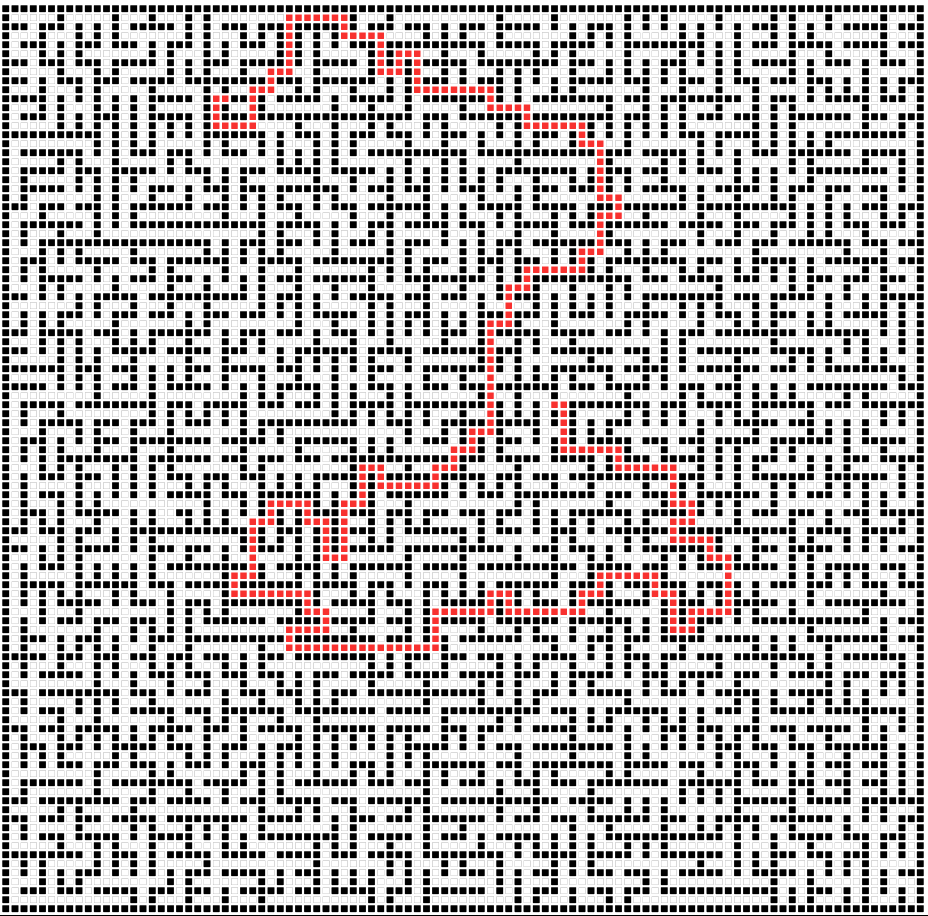
\includegraphics[width=0.6\textwidth]{pictures/single_path_maze.png}
    \caption{Single agent path planning example} 
    \label{fig:single_agent_path}
\end{figure}

In the implementation of the system, several algorithms were implemented to facilitate the efficient path planning of local agents. These included the CA*, A*, Dijkstra and Breadth-First Search (BFS) algorithms. Additionally, to support cloud-enhanced computation, the CA*, A* and Dijkstra algorithms were also implemented. The choice of algorithms was based on their computational efficiency, performance, and suitability for the specific problem domain. The system also allows for the flexibility to switch between different algorithms depending on the requirements of the specific task. Furthermore, the system was designed to be modular and extensible, allowing for the integration of additional algorithms in the future as needed by incorporating new algorithms into the existing library.

In the case of multi-agent algorithms, there are also time considerations and thus, the visualizations must include multiple time frames. To demonstrate this scenario, an example of the planned path is illustrated in Figure \ref{fig:multiple_agent_path}. The agents are not colliding, and they may choose sub-optimal paths to avoid collisions. The starting and goal positions are denoted by circles, while the agents are represented by squares.

All libraries that are necessary for the algorithms and visualizations are included during the building of the Docker image. This ensures that all required dependencies are present and that the libraries are ready for use when the image is deployed. The libraries are then imported into the main program and utilized for the functionality of the system. This approach allows for easy distribution and deployment of the system, as all necessary components are included within the Docker image and can be easily pulled and run on any system that supports Docker. Additionally, this approach ensures that the libraries are available in a consistent and predictable environment, reducing the risk of compatibility issues.

\begin{figure}[H]
    \centering
    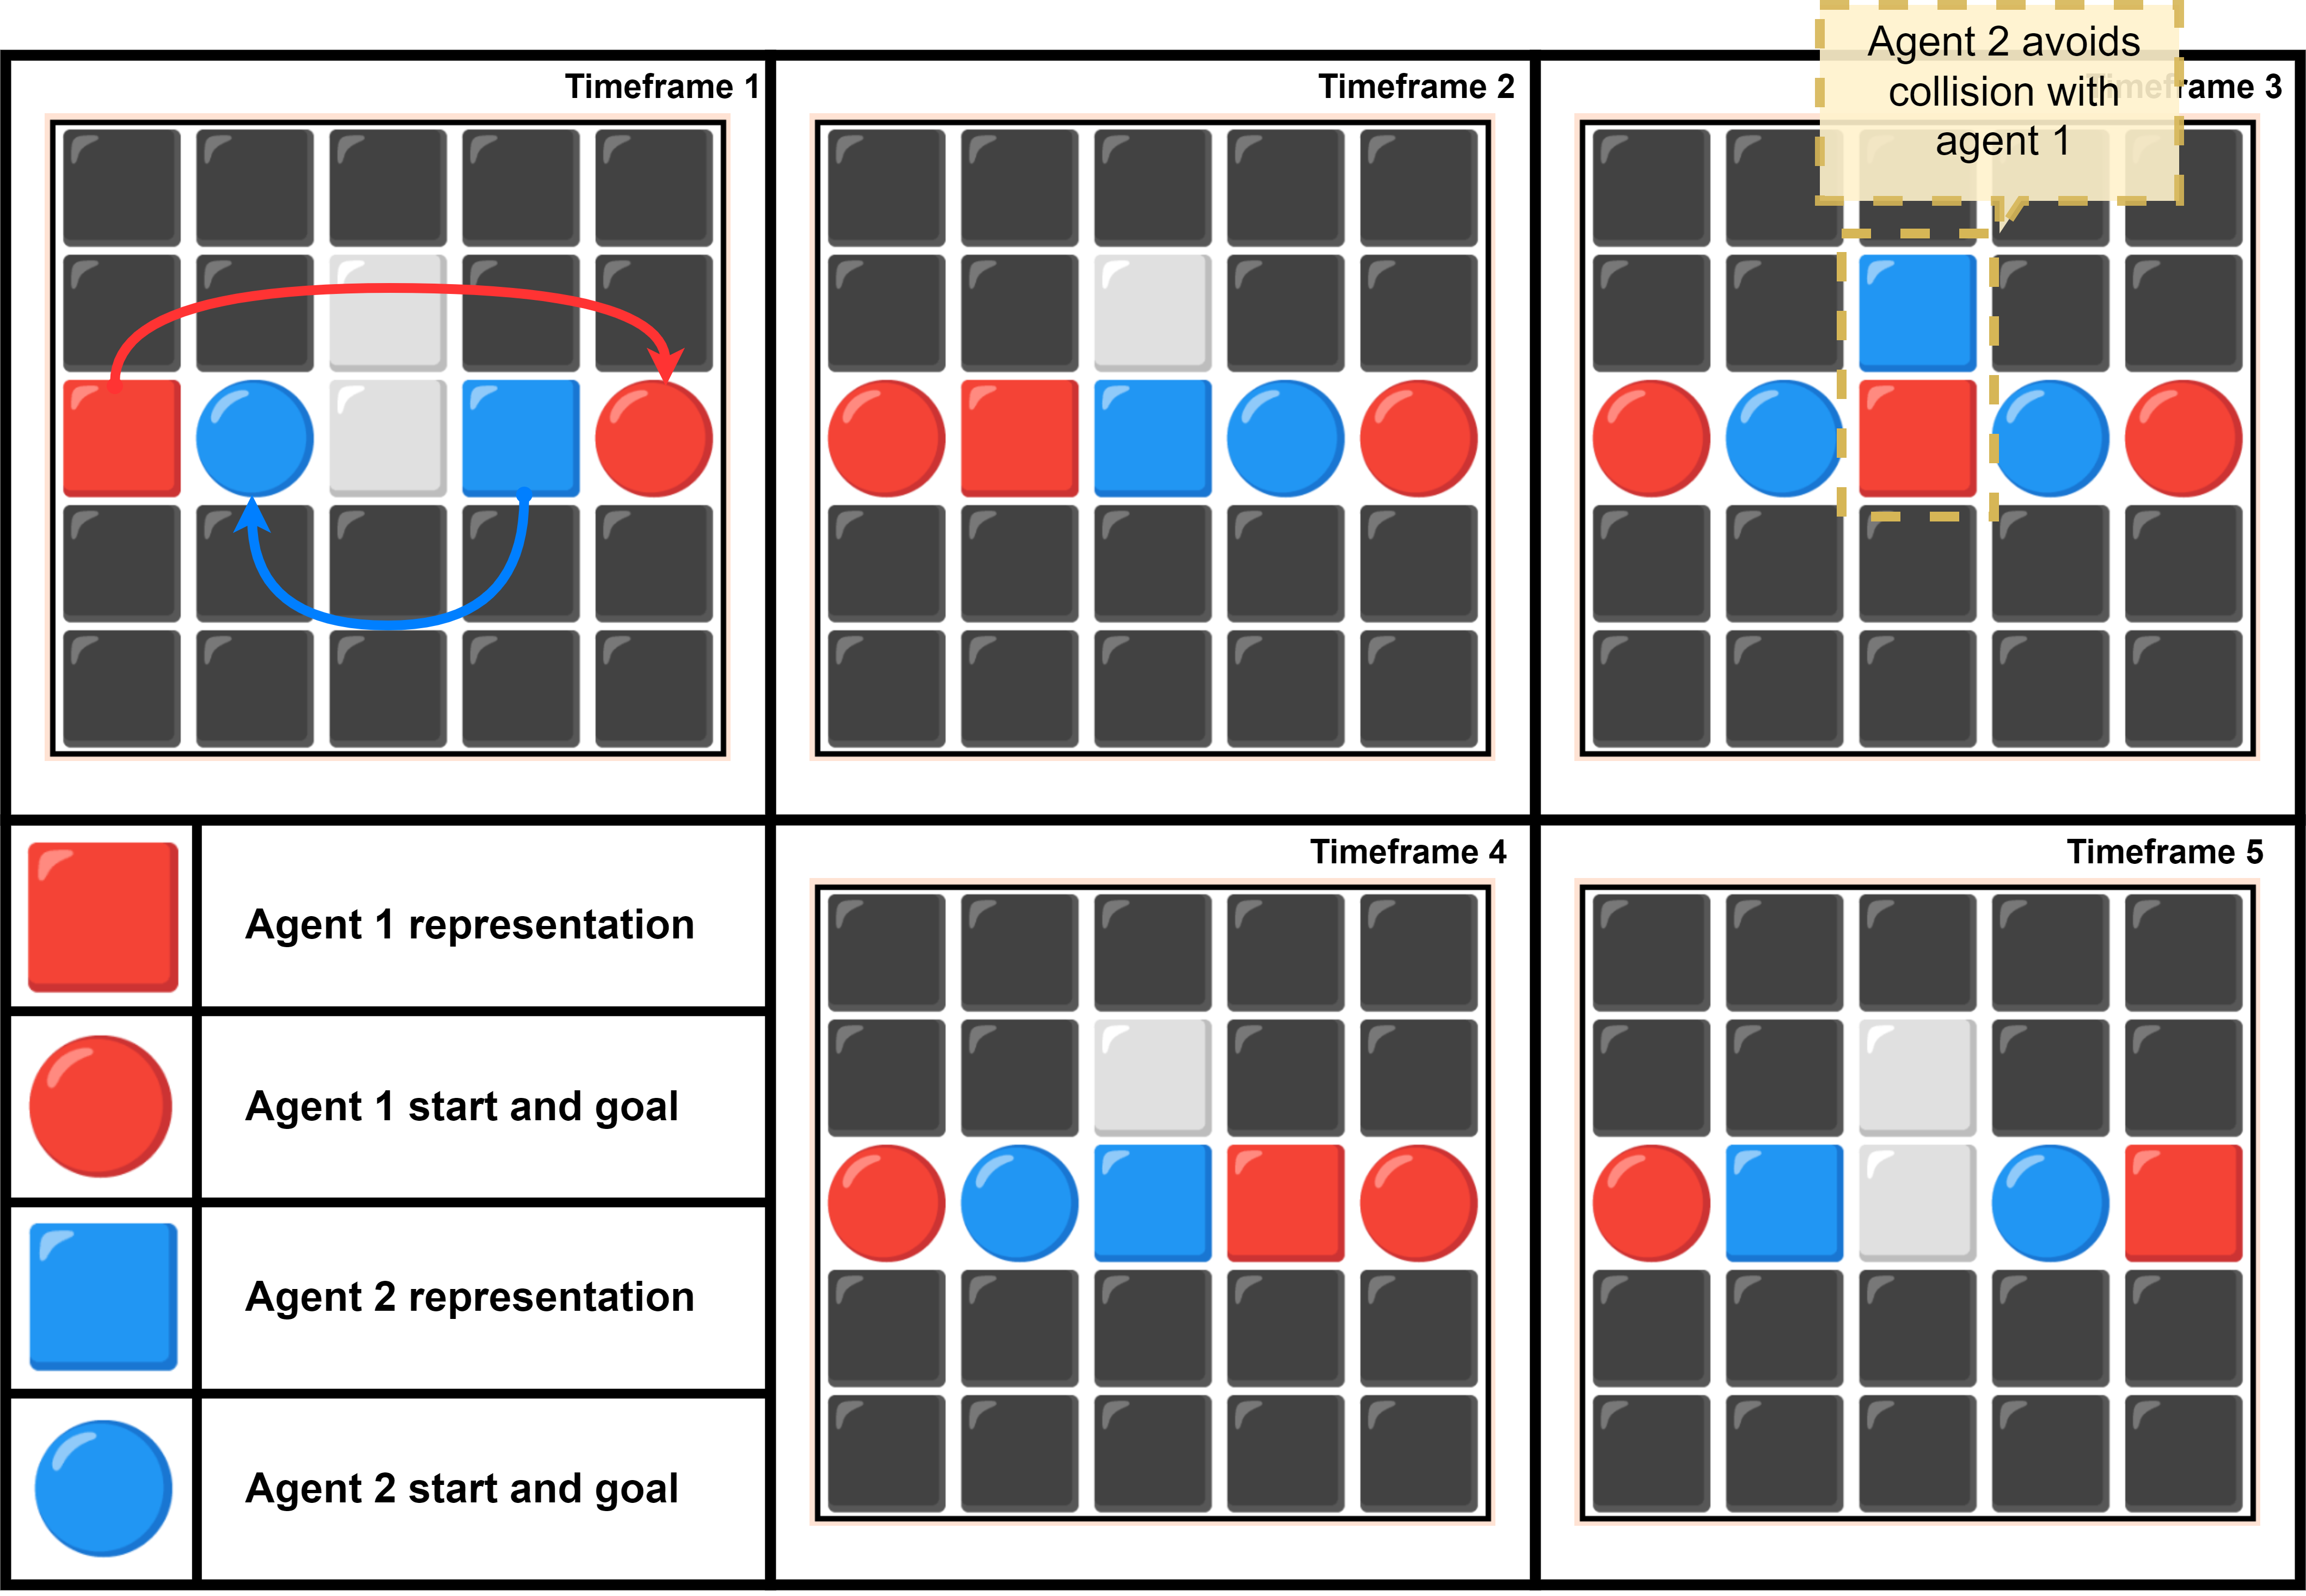
\includegraphics[width=0.9\textwidth]{pictures/example_planning.png}
    \caption{ Example of the planned path for multiple agents } 
    \label{fig:multiple_agent_path}
\end{figure}